\chapter{Metodologia}

\section{Fundamentos}

\subsection{TV Digital}

Os avanços tecnológicos dos últimos anos na área de telecomunicações têm propiciado uma melhora dos equipamentos utilizados, que, por sua vez, permitiram um enriquecimento da informação que é transmitida/recebida. Este enriquecimento nada mais é que a possibilidade de transferir mais informação num mesmo intervalo de tempo, ou seja, mais detalhes de uma mesma informação (ou uma maior qualidade dela) podem ser garantidos ao receptor ou ainda a garantia de qualidade para um número maior de receptores que compartilham um canal.

Através da transmissão digital de dados é possível atingir uma quantidade de informação transferida superior à transmissão analógica para um mesmo espectro de frequências (em grande parte devido à possibilidade de a informação digital ser comprimida), além de carregar informações (de certa forma redundantes) utilizadas para a correção de possíveis erros que possam ocorrer na transmissão devido a ruídos.

Surge deste contexto o interesse pela televisão digital em meados da década de 1970, no Japão, em que o principal objetivo era o de conseguir alta definição de imagem. Atualmente, muitos países estão num período de transição para a televisão digital, como o caso do Brasil.

A adoção da transmissão digital tem inúmeras vantagens sobre a transmissão analógica, algumas sintetizadas na Tabela \ref{tab:padroes}. Merecem destaque vantagens como a maior resolução da imagem transmitida (Full HD 1920x1080 pixels), fornecendo ao usuário uma imagem mais nítida e com muito mais detalhes; até 6 canais de áudio que permitem a utilização de equipamentos de som mais sofisticados (em comparação aos dois canais do modo estéreo da transmissão analógica); transmissão de conteúdos simultâneos por uma mesma emissora (até 6 canais em definição padrão SDTV 720x480 pixels - resolução menor que a Full HD); possibilidade de conteúdos interativos dos mais diversos e sinal livre de interferência.

\begin{table}[!htb]
	\centering
	\caption{Comparativo entre os padrões de TV}
	\label{tab:padroes}
	\begin{tabular}{lcc}
		\hline
		& \textbf{TV Analógica} & \textbf{TV Digital} \\
		\hline
		\textbf{Qualidade de imagem} & \sigla{SD}{Standard Definition} - 480 a 525 linhas & HD - até 1080 linhas \\
		\textbf{Qualidade do som} & Estéreo (2 canais) & Surround (6 canais) \\
		\textbf{Formato de exibição} & 4:3 & 16:9 \\
		\textbf{Canais por emissora} & 1 & até 6 em SD \\
		\textbf{Mobilidade} & Recepção fixa & Recepção móvel \\
		\textbf{Interatividade} & Poucas possibilidades & Muitas Possibilidades \\
		\hline
	\end{tabular}
	\fonte{\cite{tvdigitalsite}}
\end{table}

\subsection{Avaliação de vídeos}

Para que seja possível transmitir vídeos digitalmente é necessário, primeiramente, que o vídeo passe por um processo chamado codificação. O objetivo principal da codificação de vídeos é a compressão de dados que torna viável seu armazenamento e transmissão \cite{daronco}. Desta forma, a compressão tende a diminuir a fidelidade, ou seja, o problema da codificação é encontrar um compromisso entre o nível de compressão necessário para transmitir pelo canal e o nível de fidelidade que se deseja exibir para o espectador \cite{daronco}. 

Apesar de a transmissão digital garantir que a interferência à ruídos seja mínima, a qualidade da imagem não depende somente de interferência, como foi visto. A compressão de vídeos é excelente na perspectiva do transmissor já que o custo do equipamento torna-se menor, porém na perspectiva do receptor/usuário a compressão pode comprometer muito a qualidade.

Neste contexto de tentar equilibrar qualidade e compressão, surge a necessidade de se criarem métodos capazes de avaliar a qualidade dos vídeos transmitidos tanto da parte das emissoras, para saber até que ponto a compressão não é percebida pelo usuário, ou pelo menos que ela não o incomode a ponto de fazê-lo mudar de canal; quanto da parte do usuário, que colabora para ter um serviço melhor.

Diversas metodologias foram criadas para avaliar a qualidade da informação multimídia (tanto áudio quanto vídeo), divididas em dois paradigmas: avaliação objetiva e avaliação subjetiva.

A avaliação objetiva tenta, através de algoritmos, fazer uma previsão aproximada da qualidade observada pelos observadores \cite{albini}. Os métodos mais simples e mais difundidos são definidos estatisticamente como o erro médio quadrático (MSE - Mean Squared Error) e a razão sinal-ruído de pico (PSNR - Peak Signal to Noise Ratio) \cite{emmersonsilva} entre os dados originais e os dados recebidos (no caso de vídeos, o cálculo é aplicado pixel a pixel).

A avaliação subjetiva depende de observadores (humanos) que atribuem notas a partir de suas opiniões sobre a qualidade. Posteriormente, uma análise estatística dos dados coletados é realizada, resultando em uma nota chamada MOS (Mean Opinion Score) \cite{itup930} \cite{albini}. Estes tipos de avaliação possuem algumas recomendações estabelecidas por órgãos internacionais com a finalidade de padronizar os procedimentos e ambientes de avaliação, alguns exemplos destas normas podem ser observados na Tabela \ref{tab:recomendacoes}:

\begin{table}
	\centering
	\caption{Tabela de recomendações da ITU}
	\label{tab:recomendacoes}
	\begin{tabular}{c|l}
		\hline
		\textbf{Nome da Norma} & Descrição \\
		\hline
		\textbf{ITU-R Rec. BT.500} & Metodologias para avaliação subjetiva da qualidade de vídeos \\
			& em televisores \\
		\textbf{ITU-T Rec. P.910} & Métodos para avaliação subjetiva de vídeos em aplicações \\
			& multimídia \\
		\textbf{ITU-T Rec. P.911} & Métodos para avaliação subjetiva de dados audiovisuais em \\
			& aplicações multimídia \\
		\textbf{ITU-T J.144} & Técnicas para avaliação objetiva de vídeo para televisão a cabo na \\
			& na presença de uma referência \\
		\textbf{ITU-R BS.1387} & Avaliação de sistema de áudio de alta qualidade. \\
		\hline
	\end{tabular}
	\fonte{\cite{daronco}}
\end{table}

Comparando-se as metodologias, ambas são importantes e ambas têm suas limitações. A avaliação objetiva é mais precisa considerando que ela avalie a diferença entre um vídeo original e o efetivamente observado. Porém, nem sempre o vídeo original possui uma qualidade que satisfaria o telespectador, sendo esta, portanto, uma de suas desvantagens.

A avaliação subjetiva embora seja um processo mais difícil de ser realizado por depender de um grande grupo de pessoas e tenha um custo mais elevado \cite{albini}, segundo \cite{wangbovik2004} esta é o tipo de avaliação mais ‘correta’, pois o próprio telespectador realiza a avaliação.

\subsection{Vídeo digital e seus artefatos}

Imagens digitais são alvo de uma grande variedade de distorções durante sua aquisição, processamento, compressão, armazenamento, transmissão e reprodução \cite{wangbovik2004}. As características peculiares que são observadas nas imagens são chamadas de artefatos \cite{albini} e podem ser observadas tanto em transmissões digitais quanto em transmissões analógicas.

As imagens digitalmente transmitidas, embora suscetíveis à um grande número de distorções, não sofrem as mesmas distorções que as convencionais, de transmissão analógica (salvo no caso de uma imagem analógica ser convertida para ser transmitida em meio digital). O ruído branco gaussiano e o ruído sal e pimenta são exemplos de distorções que ocorrem em meio analógico e podem ser observados na Figura~\ref{fig:artefatosanalogicos} a seguir:

\begin{figure}[!htb]
	\centering
	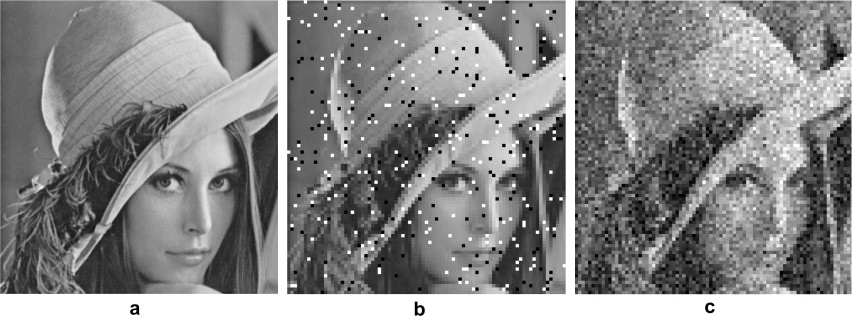
\includegraphics[width=0.8\textwidth]{./imgs/figura0.png}
	\caption{Artefatos em vídeos analógicos: (a) imagem original, (b) ruído sal e pimenta e (c) ruído branco gaussiano.}
	\label{fig:artefatosanalogicos}
	\fonte{\cite{panagiotopoulou}}
\end{figure}

Em se tratando de vídeos digitais, os artefatos de maior notoriedade são: blocagem, borramento, efeito vibrante e ruído (blockiness, blurriness, ringing, e noisiness) \cite{farias2007}. Estes efeitos podem ser observados na Figura~\ref{fig:artefatosdigitais}, a seguir:

\begin{figure}[!htb]
	\centering
	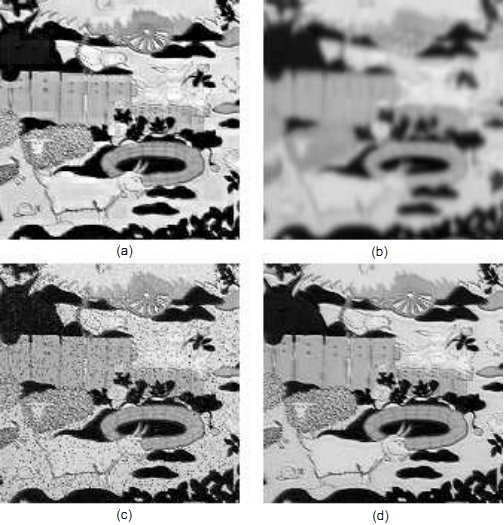
\includegraphics[scale=0.45]{./imgs/figura1.png}
	\caption{Principais artefatos em vídeos digitais: (a) blocagem; (b) borramento; (c) ruído e (d) efeito vibrante.}
	\label{fig:artefatosdigitais}
	\fonte{\cite{farias2007}}
\end{figure}


Poder adicionar artefatos de forma artificial e controlada à vídeos digitais é de grande importância no campo de avaliação de vídeos (tanto na avaliação objetiva quanto na avaliação subjetiva) uma vez que, a partir de algoritmos, é possível simular distorções reais. Estes algoritmos não são padronizados, mas existem algumas recomendações internacionais, como por exemplo a recomendação P.930 da ITU \cite{itup930} que descreve os princípios para reproduzir as distorções relativas à compressão de vídeo sem efetivamente precisar comprimí-lo.

\section{Processo de desenvolvimento}
O desenvolvimento do presente trabalho..

\begin{table}
	\centering
	\caption{Tabela de fases do desenvolvimento}
	\label{tab:metodologia}
	\begin{tabular}{c|l}
	\hline
	\textbf{Fase} & \textbf{Descrição} \\
	\hline
	\textbf{1.} & 1. Revisão bibliográfica, compreensão de conceitos \\
		& 2. Análise do SASQV \\
	\textbf{1,5.} & 1. Levantamento de requisitos \\
	\textbf{2.} & 1. Desenvolvimento das ferramentas de degradação \\
		& 2. Desenvolvimento da interface \\
	\textbf{3.} & 1. Teste e validação das Ferramentas. \\
		& 2. Testes da Interface \\
	\textbf{4.} & 1. Integração: ferramentas e interface \\
	\textbf{5.} & 1. Geração e avaliação de uma base de vídeos \\
	\hline
	\end{tabular}
\end{table}	
